% !TEX encoding = ITF-8 Unicode
%
% Niniejszy plik stanowi przykład formatowania pracy magisterskiej na
% Wydziale MIM UW.  Szkielet użytych poleceń można wykorzystywać do
% woli, np. formatujac wlasna prace.
%
% Zawartosc merytoryczna stanowi oryginalnosiagniecie
% naukowosciowe Marcina Wolinskiego.  Wszelkie prawa zastrzeżone.
%
% Copyright (c) 2001 by Marcin Woliński <M.Wolinski@gust.org.pl>
% Poprawki spowodowane zmianami przepisów - Marcin Szczuka, 1.10.2004
% Poprawki spowodowane zmianami przepisow i ujednolicenie 
% - Seweryn Karłowicz, 05.05.2006
% dodaj opcję [licencjacka] dla pracy licencjackiej
\documentclass{pracamgr}

\usepackage{polski}

%Jesli uzywasz kodowania polskich znakow ISO-8859-2 nastepna linia powinna byc 
%odkomentowana
%\usepackage[latin2]{inputenc}
%Jesli uzywasz kodowania polskich znakow CP-1250 to ta linia powinna byc 
%odkomentowana
\usepackage[utf8]{inputenc}
\RequirePackage{graphicx}
\RequirePackage{longtable}
\usepackage[usenames,dvipsnames]{color}
\usepackage{subfigure}
%\usepackage{hyperref}
%\usepackage{url}
\definecolor{gray}{RGB}{50,50,50}

\usepackage[colorlinks=true,linkcolor=gray,urlcolor=blue]{hyperref}  



\newcommand{\emptyP}{\mbox{$\epsilon$}}
\newcommand{\terminal}[1]{\mbox{{\texttt {#1}}}}
\newcommand{\nonterminal}[1]{\mbox{$\langle \mbox{{\sl #1 }} \! \rangle$}}
\newcommand{\arrow}{\mbox{::=}}
\newcommand{\delimit}{\mbox{$|$}}
\newcommand{\reserved}[1]{\mbox{{\texttt {#1}}}}
\newcommand{\literal}[1]{\mbox{{\texttt {#1}}}}
\newcommand{\symb}[1]{\mbox{{\texttt {#1}}}}
% Dane magistranta:

\author{Imię i nazwisko}

\nralbumu{nralbumu}

\title{Intuicyjny język wyszukiwania TQL (Tablets Query Language)}

\tytulang{Intuitive query language TQL (Tablets Query Language)}

%kierunek: Matematyka, Informatyka, ...
\kierunek{Informatyka}

% informatyka - nie okreslamy zakresu (opcja zakomentowana)
% matematyka - zakres moze pozostac nieokreslony,
% a jesli ma byc okreslony dla pracy mgr,
% to przyjmuje jedna z wartosci:
% {metod matematycznych w finansach}
% {metod matematycznych w ubezpieczeniach}
% {matematyki stosowanej}
% {nauczania matematyki}
% Dla pracy licencjackiej mamy natomiast
% mozliwosc wpisania takiej wartosci zakresu:
% {Jednoczesnych Studiow Ekonomiczno--Matematycznych}

% \zakres{Tu wpisac, jesli trzeba, jedna z opcji podanych wyzej}

% Praca wykonana pod kierunkiem:
% (podać tytuł/stopień imię i nazwisko opiekuna
% Instytut
% ew. Wydział ew. Uczelnia (jeżeli nie MIM UW))
\opiekun{dra Roberta Dąbrowskiego\\
  Instytut Informatyki\\
  }

% miesiąc i~rok:
\date{czerwiec 2010}

%Podać dziedzinę wg klasyfikacji Socrates-Erasmus:
\dziedzina{ 
%11.0 Matematyka, Informatyka:\\ 
%11.1 Matematyka\\ 
%11.2 Statystyka\\ 
11.3 Informatyka\\ 
%11.4 Sztuczna inteligencja\\ 
%11.5 Nauki aktuarialne\\
%11.9 Inne nauki matematyczne i informatyczne
}

%Klasyfikacja tematyczna wedlug AMS (matematyka) lub ACM (informatyka)
\klasyfikacja{H. INFORMATION SYSTEMS\\
H.2. DATABASE MANAGEMENT\\
H.2.3 Languages}

% Słowa kluczowe:
\keywords{}

% Tu jest dobre miejsce na Twoje własne makra i~środowiska:
\newtheorem{defi}{Definicja}[section]

% koniec definicji

\begin{document}
\maketitle

%tu idzie streszczenie na strone poczatkowa
\begin{abstract}
Sumerologia jest dziedziną badań nad antycznym językiem Sumerów, w której
kluczowym zagadnieniem jest przeszukiwanie dużych zbiorów informacji
zapisanych na odnalezionych tabliczkach sumeryjskich.

W pracy przedstawiono definicję przeznaczonego dla sumerologów intuicyjnego
języka przeszukiwania zbiorów tabliczek (Tablets Query Language) wraz z jego
przykładową implementacją opartą na relacyjnej bazie danych.

%TODO: drugi intuicyjny
Celem tej pracy jest stworzenie języka zapytań intuicyjnego dla sumerologów,
stanowiącego znaczące uproszczenie w stosunku do SQL dzięki wprowadzeniu pojęć 
naturalnych dla rozważanej dziedziny. Jednocześnie TQL nadal
pozwala na tworzenie skomplikowanych zapytań wyszukujących, natomiast nie 
udostępnia funkcji tworzących i modyfikujących bazę. Można go rozszerzać 
i zmieniać tak, by mógł służyć też do innych zastosowań.
\end{abstract}

\tableofcontents
%\listoffigures
%\listoftables


\chapter*{Wprowadzenie}
\addcontentsline{toc}{chapter}{Wprowadzenie}
%  \begin{figure}
%   \centering
% \includegraphics[width=340px]{./diagramy/poco.pdf}
%   \caption{Zarysowanie problemu}
%  \end{figure}
\begin{figure}[h]
 \centering
 \includegraphics[width=400px]{../diagramy/poco.pdf}
 % poco.pdf: 596x842 pixel, 72dpi, 21.03x29.70 cm, bb=0 0 596 842
 \caption{Przedstawienie problemu}
 \label{fig:poco}
\end{figure}

 
 
Niniejsza praca dotyczy problemu przetwarzania baz danych tabliczek sumeryjskich przez osoby nieznające specyficznych dla baz danych języków zapytań.


Istnieje wiele baz danych zawierających teksty odczytane z tabliczek sumeryjskich (najbardziej znana - CDLI zawiera ich prawie 225 tys.). Sumerolodzy zajmują się badaniem i przetwarzaniem tych tekstów, jednak wyszukiwanie interesujących ich tabliczek jest dosyć niewygodne. Wynika to przede wszystkim z nieznajomości specyficznych dla baz danych języków zapytań. 
Większość serwisów internetowych udostępnia formularze ułatwiające wprowadzanie kryteriów wyszukiwania, jednakże mają one ograniczone możliwości (nie pozwalają na skomplikowane konstrukcje). Dlatego istnieje potrzeba stworzenia narzędzia, które będzie łączyło w sobie jak największą siłę wyrazu i łatwość użycia przez osoby znające jedynie dziedzinę problemu. Celem projektu przedstawionego w niniejszej pracy jest zaprojektowanie i implementacja języka Tablets Query Language (TQL) spełniającego powyższe wymagania. 

TQL jest podstawą do tworzenia podobnych języków wyszukiwań dostosowanych do potrzeb innych grup ludzi, np. językoznawców.
Większość programów ułatwiających tworzenie zapytań jest skomplikowana, daje ograniczone możliwości lub jest przystosowana głównie do przetwarzania danych liczbowych. Tablets Query Language rozwiązuje te problemy: jest prosty i intuicyjny, przystosowany głównie do tekstów, minimalnie zmniejsza siłę wyrazu oraz łatwo go rozbudowywać. 

%Język TQL jest nakładką na inne języki (m.in. SQL). 
Zgodnie z paradygmatem języków dziedzinowych (Domain Specific Languages, DSL) TQL jest nakładką na inne języki zapytań (np. SQL).
% TQL jest jednym z języków dziedzinowych (Domain Specific Languages, DSL). 
W związku z tym dla każdego sposobu reprezentacji danych należy skonstruować translator, 
którego zadaniem będzie przetłumaczenie zapytania. 
% Dla każdego z nich, w zależności od reprezentacji danych, należy skonstruować translator, 
% którego zadaniem będzie przetłumaczenie zapytania. 
W ramach niniejszej pracy przedstawione zostaną dwa przykładowe translatory.

\chapter{Podstawowe pojęcia}\label{r:pojecia}
\section{Definicje}
\begin{description}
 \item[Sumerolodzy] - ludzie, którzy zajmują się odczytywaniem pisma klinowego w języku sumeryjskim. Na potrzeby tej pracy
		      to pojęcie jest rozszerzone do wszystkich ludzi zajmujących się odczytywaniem tabliczek sumeryjskich 
		      i wyciąganiem z nich wiedzy historycznej.
 \item[Tabliczka] - w tej pracy tabliczka będzie oznaczała tabliczkę sumeryjską w wersji elektronicznej 
		  (chyba, że zostanie zaznaczone inaczej). Dla rozróżnienia, kiedy będziemy mówić o ``prawdziwej'', 
		  glinianej tabliczce, będziemy używać pojęcia \textbf{gliniana tabliczka}
 \item[Prowiniencja] - pojęcie używane przez sumerologów, oznacza miejsce pochodzenia/znalezienia glinianej tabliczki
 \item[Kliny] - znaki występujące na glinianych tabliczkach.
 \item[Odczyty] - sposób transkrypcji klinów, występuje na tabliczkach elektronicznych.
 \item[Pieczęć] - część tabliczki zawierająca znak rozpoznawczy autora
\end{description}



\chapter{Wcześniejsze rozwiązania}\label{r:losers}
W chwili obecnej nie ma czegoś takiego jak język dostosowany do potrzeb sumerologów. 
Są strony internetowe oferujące wyszukiwanie za pomocą formularzy.
\section{The Cuneiform Digital Library Initiative \cite{cdli}}
\begin{figure}[h]
 \centering
 \includegraphics[width=300px]{../diagramy/cdli-search.png}
 % cdli-search.png: 877x501 pixel, 72dpi, 30.94x17.67 cm, bb=0 0 877 501
 \caption{Formularz wyszukiwania na CDLI}
 \label{fig:cdli-search}
\end{figure}

Największa znana nam baza tekstów sumeryjskich (ok. 225 tys. tekstów), 
wyszukiwanie po praktycznie wszystkich możliwych parametrach, choć trochę mało wygodne. 
Dla każdej metadanej jest pole tekstowe z możliwymi opcjami wyszukiwania: ``begins with``, ``contains'', ''does not contain''. 
Dla treści jest pole tekstowe z opcjami ``word``, ``part of word`` oraz checkbox ''advanced search syntax''. 
Brakuje wyjaśnienia jak 
używać ``Advanced search syntax'' oraz możliwości tworzenia złożonych zapytań.

\section{The Electronic Text Corpus of Sumerian Literature \cite{etcsl}} 
\begin{figure}[h]
 \centering
 \includegraphics[width=300px]{../diagramy/etcsl-search.png}
 % etcsl-search.png: 774x182 pixel, 72dpi, 27.31x6.42 cm, bb=0 0 774 182
 \caption{Formularz wyszukiwania na etcsl}
 \label{fig:etcsl-search}
\end{figure}

Baza znacznie mniejsza, zawiera 
głównie teksty literackie. Wyszukiwanie mało rozbudowane. Można wybrać:
\begin{itemize}
 \item typ wyszukiwanego słowa (form, lemma, label, pos, emesal, sign)
 \item sortowanie
 \item kategorię (ponad 20 kategorii)
 \item sposób wyświetlania wyników
\end{itemize}

Można zadać zapytanie z kilkoma słowami różnych typów, można określić czy słowo ma być rzeczownikiem, imieniem boga itp. Można też pytać o część słowa.
\chapter{Dziedzina problemu}

\begin{wrapfigure}{R}{3in}
%%%%%%%%%%%%%%%%%%%%%%%%%%%%%%%%%%%%%%%%%%%%%%%%%%%%%%%%%%%%%%%%%%%%%%%%%%%%%%%%%%%%%%%
%%% You will need to add \usepackage{wrapfig} to your preamble to use textwrapping %%%
%%%%%%%%%%%%%%%%%%%%%%%%%%%%%%%%%%%%%%%%%%%%%%%%%%%%%%%%%%%%%%%%%%%%%%%%%%%%%%%%%%%%%%%
 \centering
 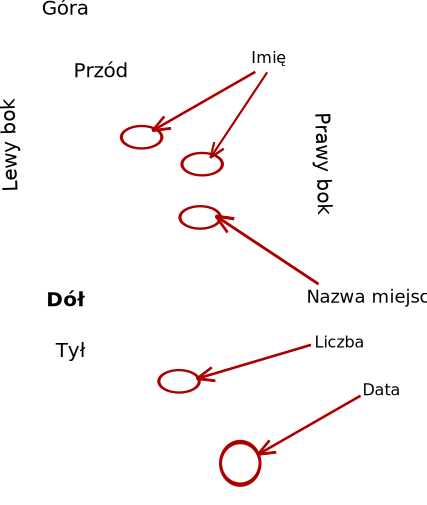
\includegraphics[width=150px]{../diagramy/tabliczka.pdf}
 % tabliczka.pdf: 342x405 pixel, 72dpi, 12.06x14.29 cm, bb=0 0 342 405
 \caption{Gliniana tabliczka - struktura}
\end{wrapfigure}


% \begin{figure}[h]
%  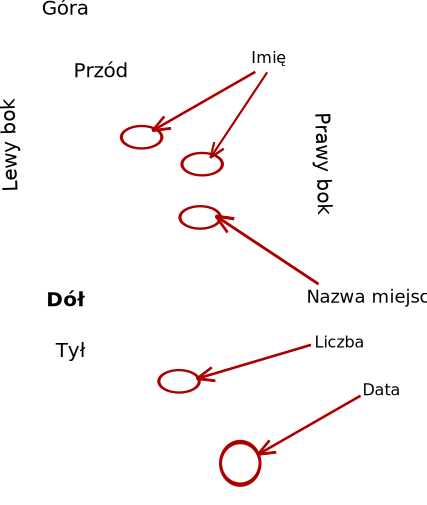
\includegraphics[width=150px]{../diagramy/tabliczka.pdf}
%  % tabliczka.pdf: 342x405 pixel, 72dpi, 12.06x14.29 cm, bb=0 0 342 405
%  \caption{Gliniana tabliczka - struktura}
% \end{figure}

\begin{figure}
 \centering
 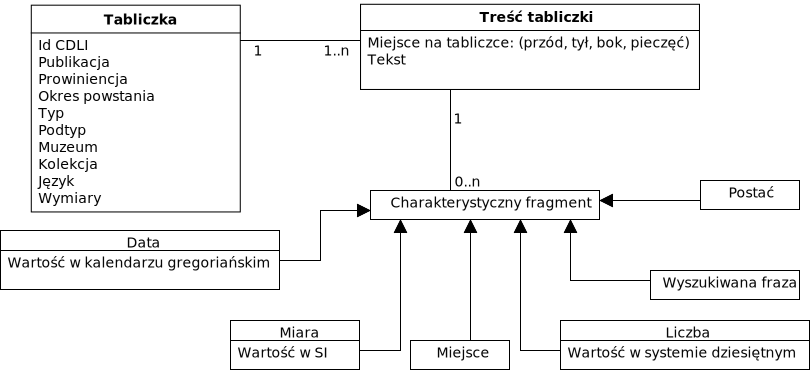
\includegraphics[width=400px]{../diagramy/Model-dziedziny.pdf}
 % Model-dziedziny.png: 650x345 pixel, 72dpi, 22.93x12.17 cm, bb=0 0 650 345
 \caption{Co powinna zawierać tabliczka w formie elektronicznej}
\end{figure}
~ 

Głównym pojęciem dziedziny jest tabliczka rozumiana dwojako - jako fizyczna tabliczka gliniana lub jako tabliczka w formie cyfrowej. 
Jej najważniejszym elementem jest treść zapisana klinami (w tabliczce glinanej) lub odczytami (w tabliczce elektronicznej), która 
może zawierać m. in. imiona
osób lub bóstw, liczby, jednostki (np. przy opisywaniu wypłat), miejsca, daty. 
Część tych elementów można przetłumaczyć na 
współczesny język (np. jednostki przeliczyć na SI, datę opisową na datę liczbową BC). 
Ponadto gliniane tabliczki są zapisywane z różnych stron 
(od góry, z przodu, z tyłu itp) oraz mogą zawierać pieczęcie - co znajduje odzwierciedlenie w treści tabliczki elektronicznej. 

Niestety odczyty zawarte w cyfrowym zapisie tabliczki są tylko jednym z wariantów tłumaczenia z klinów. 
Ponieważ w cyfrowej wersji nie ma klinów, możliwe są pomyłki w tłumaczeniach, które ciężko zweryfikować.
Choć są one dosyć mało prawdopodobne, sumerolodzy chcieliby mieć możliwość wyszukiwania po alternatywnych tłumaczeniach.

% Są też uszkodzone fragmenty, które zostały cyfrowo zapisane w najróżniejszej formie.

Poza treścią tabliczki cyfrowa wersja zawiera także metadane informujące m. in. o jej miejscu znalezienia, czasie powstania, 
 kolekcji do której obecnie należy, publikacji, w której się pojawiła. 
Są one istotne, gdyż często pozwalają na określenie o czym jest tabliczka bez dokładnej analizy jej treści. 
Jednym z atrybutów, który w znacznym stopniu pomaga zidentyfikować tabliczkę jest publikacja.



%TODO:spytać
% Sumerolodzy potrafią określić w przybliżeniu treść tabliczki na podstawie publikacji.
%TODO:ciągłość

Sumerolodzy oczekują możliwości wyszukiwania po metadanych, po treści tabliczki (po odczytach) 
i po alternatywnych tłumaczeniach (po klinach).  %TODO: po klinach??
Dodatkową zaletą byłoby wyszukiwanie po tagach (imionach, jednostkach, datach itp)
W pierwszej wersji języka implementujemy tylko wyszukiwanie po odczytach i metadanych.
\chapter{Definicja języka TQL}
\section{Tablets Query Language}
Tablets Query Language (TQL) jest naszą propozycją rozwiązania problemu wyszukiwania tabliczek sumeryjskich.
Jest to zewnętrzny język dziedzinowy stworzony do tego, aby służyć sumerologom jako język zapytań.
Formalna definicja składni TQL znajduje się w rozdziale \ref{chap:skladnia}.
Jest ona zaprojektowana od podstaw, dzięki czemu jest bardzo prosta i intuicyjna, co będzie widać na przykładach 
opisujących semantykę w rozdziale \ref{chap:semantyka}. 
Wiele języków dziedzinowych, w przeciwieństwie do TQL, bazuje na istniejących już językach. Są to tzw. wewnętrzne języki dziedzinowe. Jednak w przypadku naszego problemu było to niewskazane rozwiązanie, gdyż składnia przejęta z istniejącego języka zapytań bardziej ogólnego zastosowania byłaby nieintuicyjna, a tworzone zapytania długie i skomplikowane.
Udało nam się połączyć prostą składnię TQL z dużą siłą wyrazu.
 Język daje możliwość formułowania złożonych 
wyrażeń do wyszukiwania na podstawie pojedynczej
metadanej lub treści tabliczki oraz możliwość łączenia wielu zapytań w jedno.

Dodatkowo, jednym z głównych założeń przyjętych przy tworzeniu języka TQL jest niezależność od rzeczywistej
reprezentacji danych. Przy konstruowaniu go nie brałyśmy pod uwagę sposobu fizycznej reprezentacji tabliczek,
czyli rodzaju bazy danych oraz schematu danych. Skupiłyśmy się jedynie na dziedzinie problemu, czyli na tym,
co zawiera tabliczka oraz na podstawie jakich informacji chcemy wyszukiwać. Zakładamy, że niezależnie od
reprezentacji danych takie wyszukiwanie będzie możliwe, chociaż oczywiście skonstruowanie odpowiedniego
zapytania może być skomplikowane. Przetłumaczenie zapytania TQL na zapytanie w języku odpowiednim do
reprezentacji danych, np. SQL, XQuery, jest zadaniem programu tłumaczącego. Dzięki temu praca polegająca
na przetłumaczeniu zapytania z "języka dziedziny" na "język komputerów" jest wykonana tylko raz dla każdego
sposobu reprezentacji danych, i to przez programistów, a nie sumerologów.

Język TQL umożliwia wyszukiwanie na podstawie kryteriów dotyczących następujących danych:
\begin{longtable}{|p{3in}|p{2.5in}|}
\hline
{\bf Opis} & {\bf Nazwa pola w TQL}\\
\hline
\endhead
numer tabliczki w bazie CDLI & cdli\_id
\\
\hline
miejsce pochodzenia (proweniencja) & provenience
\\
\hline
okres powstania & period
\\
\hline
typ i podtyp & genre
\\
\hline
rok powstania & year
\\
\hline
publikacja & publication
\\
\hline
treść (odczyty)& text
\\
\hline
%treść (kliny) & cunetext
%\\
%\hline
kolekcja & collection
\\
\hline
muzeum & museum
\\
\hline
\end{longtable}
Język można łatwo rozszerzać, aby umożliwić tworzenie kryteriów wyszukiwania w oparciu o inne dane
(np. kliny, zawartość pieczęci).

W kolejnych dwóch rozdziałach przedstawimy gramatykę i semantykę zaprojektowanego przez nas języka TQL.



\section{\label{chap:skladnia}Gramatyka}

W tym rozdziale przedstawimy gramatykę zaprojektowanego przez nas języka.
W pierwszej części pokażemy strukturę leksykalną TQL, czyli elementy, z których buduje się zapytania.
W drugiej części zaprezentujemy reguły tworzenia zapytań, zapisane w formie reguł gramatyki w notacji BNF.

\subsection{Struktura leksykalna}

\subsubsection{Literały}

% \paragraph{String}
Literał \terminal{String}\ jest ciągiem dowolnych znaków w cudzysłowie (\texttt{"}). Nie może zawierać jedynie znaków
``\texttt{"}`` niepoprzedzonych ''\verb6\6``.

% \paragraph{SłowoOdLitery}
Literał \terminal{SłowoOdLitery} to ciąg liter, cyfr oraz znaków {''\texttt{-}``, ''\texttt{'}``, ''\texttt{\_}``},
zaczynający się od litery, z wyjątkiem słów kluczowych.

% \paragraph{SłowoOdLiczby}
Literał \terminal{SłowoOdLiczby} to ciąg liter, cyfr oraz znaków {''\texttt{-}``, ''\texttt{'}``, ''\texttt{\_}``},
zaczynający się od cyfry.


\subsubsection{Słowa kluczowe}

\begin{tabular}{lll}
{\reserved{as}} &{\reserved{define}} &{\reserved{in}} \\
{\reserved{search}} & & \\
\end{tabular}\\

\subsubsection{Znaki specjalne}

\begin{tabular}{lll}
{\symb{(}} &{\symb{)}} &{\symb{{$+$}}} \\
{\symb{/}} &{\symb{{$-$}{$-$}}} &{\symb{*}} \\
{\symb{:}} & &{\symb{$\backslash$n}} (koniec linii)\\
\end{tabular}\\

\subsection{\label{sec:skladnia}Struktura składniowa języka}

Poniżej przedstawimy reguły gramatyki TQL w notacji BNF.
Nieterminale są zapisane pomiędzy ''$\langle$`` a ''$\rangle$``.
Symbole ''{\arrow}`` (produkcja), ''{\delimit}`` (lub)
i ''{\emptyP}`` (pusta reguła) należą do notacji BNF.
Wszystkie pozostałe symbole to terminale.\\

\begin{tabular}{lll}
{\nonterminal{Zapytanie Złożone}} & {\arrow} &{\nonterminal{Lista Zapytań}} \\
\end{tabular}\\

\begin{tabular}{lll}
{\nonterminal{Lista Zapytań}} & {\arrow} &{\nonterminal{Zapytanie}} \\
 & {\delimit} &{\nonterminal{Zapytanie}} {\nonterminal{Lista Zapytań}} \\
\end{tabular}\\

\begin{tabular}{lll}
{\nonterminal{Zapytanie}} & {\arrow} &{\nonterminal{Lista Linii Zapytania}} {\nonterminal{Lista Pustych Linii}} \\
 & {\delimit} &{\terminal{define}} {\terminal{$\backslash$n}} {\nonterminal{Zapytanie}} {\terminal{as}} {\nonterminal{Nazwa}} {\nonterminal{Lista Pustych Linii}} \\
 & {\delimit} &{\terminal{search}} {\terminal{$\backslash$n}} {\nonterminal{Zapytanie}} {\terminal{in}} {\nonterminal{Nazwa}} {\nonterminal{Lista Pustych Linii}} \\
  & {\delimit} &{\terminal{search}} {\nonterminal{Nazwa}} {\nonterminal{Lista Pustych Linii}} \\
 & {\delimit} &{\nonterminal{Lista Pustych Linii}} \\
\end{tabular}\\

\begin{tabular}{lll}
{\nonterminal{Lista Linii Zapytania}} & {\arrow} &{\nonterminal{Linia Zapytania}} {\terminal{$\backslash$n}} \\
 & {\delimit} &{\nonterminal{Linia Zapytania}} {\terminal{$\backslash$n}} {\nonterminal{Lista Linii Zapytania}} \\
\end{tabular}\\

\begin{tabular}{lll}
{\nonterminal{Linia Zapytania}} & {\arrow} &{\nonterminal{Nazwa pola}} {\terminal{:}} {\nonterminal{Wyrażenie}} \\
\end{tabular}\\

\begin{tabular}{lll}
{\nonterminal{Wyrażenie}} & {\arrow} &{\nonterminal{Wyrażenie}} {\terminal{{$+$}}} {\nonterminal{Wyrażenie1}} \\
 & {\delimit} &{\nonterminal{Wyrażenie}} {\terminal{/}} {\nonterminal{Wyrażenie1}} \\
 & {\delimit} &{\nonterminal{Wyrażenie1}} \\
\end{tabular}\\

\begin{tabular}{lll}
{\nonterminal{Wyrażenie1}} & {\arrow} &{\terminal{{$-$}{$-$}}} {\nonterminal{Wyrażenie1}} \\
 & {\delimit} &{\nonterminal{Wyrażenie2}} \\
\end{tabular}\\

\begin{tabular}{lll}
{\nonterminal{Wyrażenie2}} & {\arrow} &{\nonterminal{Wyrażenie3}} {\terminal{*}} {\nonterminal{Wyrażenie3}} \\
 & {\delimit} &{\nonterminal{Tekst}} \\
 & {\delimit} &{\terminal{(}} {\nonterminal{Wyrażenie}} {\terminal{)}} \\
\end{tabular}\\

\begin{tabular}{lll}
{\nonterminal{Wyrażenie3}} & {\arrow} &{\nonterminal{Wyrażenie2}}\\
 & {\delimit} &{\emptyP} \\
\end{tabular}\\

\begin{tabular}{lll}
{\nonterminal{Lista Pustych Linii}} & {\arrow} &{\emptyP} \\
 & {\delimit} &{\nonterminal{Pusta Linia}} {\nonterminal{Lista Pustych Linii}} \\
\end{tabular}\\

\begin{tabular}{lll}
{\nonterminal{Pusta Linia}} & {\arrow} &{\terminal{$\backslash$n}} \\
\end{tabular}\\

\begin{tabular}{lll}
{\nonterminal{Tekst}} & {\arrow} &{\terminal{String}} \\
 & {\delimit} &{\nonterminal{Słowo}} \\
\end{tabular}\\

\begin{tabular}{lll}
{\nonterminal{Słowo}} & {\arrow} &{\terminal{SłowoOdLitery}} \\
 & {\delimit} &{\terminal{SłowoOdLiczby}} \\
\end{tabular}\\

\begin{tabular}{lll}
{\nonterminal{Nazwa pola}} & {\arrow} &{\terminal{SłowoOdLitery}} \\
\end{tabular}\\

\begin{tabular}{lll}
{\nonterminal{Nazwa}} & {\arrow} &{\terminal{String}} \\
\end{tabular}\\

Powyższa gramatyka jest gramatyką bezkontekstową.

\section{\label{chap:semantyka}Semantyka}

Poniżej przedstawiamy semantykę wybranych przykładów.
\subsection{Zapytanie proste}
\begin{verbatim}
provenience: Gar*
period: "Ur III"
genre: Administrative
text: udu + (masz2/ugula) --szabra
\end{verbatim}
Wynikiem zapytania będą wszystkie tabliczki, które:
\begin{itemize}
\item pochodzą z miejscowości o nazwie zaczynającej się na ``Gar''
\item pochodzą z okresu Ur III
\item są dokumentami administracyjnymi
\item zawierają słowo ``udu'' oraz conajmniej jedno ze słów ``masz2'' lub ``ugula''
\item nie zawierają słowa ``szabra''.
\end{itemize}


\subsection{Zapytanie złożone}
\begin{verbatim}
provenience: Ur
period: "Ur III"/"Ur IV"
text: udu --szabra

text: masz2/ugula
publication: *tan
provenience: Ur
\end{verbatim}
Wynikiem zapytania będą wszystkie tabliczki, które:
\begin{itemize}
 \item pochodzą z miejscowości Ur
 \item pochodzą z okresu Ur III lub Ur IV
 \item zawierają słowo ``udu''
 \item nie zawierają słowa ``szabra``
\end{itemize}
oraz wszystkie tabliczki, które:
\begin{itemize}
 \item zawierają słowo ''masz2`` lub ''ugula``
 \item zostały opublikowane w pracy, której nazwa kończy się na ''tan``
 \item pochodzą z miejscowości Ur.
\end{itemize}


\subsection{\label{sec:zdefiniowane} Zapytanie zdefiniowane}
\begin{verbatim}
 define
  provenience: Gar*a
  period: Ur III
  text: "udu ban"/mash2
as "zwierzęta w Gar*a"
\end{verbatim}
Wynikiem zapytania (po jego wywołaniu) będą wszystkie tabliczki, które:
\begin{itemize}
\item pochodzą z miejscowości, których nazwy zaczynają się na ''Gar`` i kończą na ''a''
\item pochodzą z okresu Ur III
\item zawierają conajmniej jedną z fraz ''udu ban`` lub ''mash2``.
\end{itemize}

\subsection{Wywołanie zapytania zdefiniowanego}
\subsubsection{Zwykłe}
\begin{verbatim}
search "zwierzęta w Gar*a"
\end{verbatim}
Wynikiem zapytania będą dokładnie te tabliczki, które spełniają wszystkie warunki zapytania ''zwierzęta w Gar*a``.\\
Takie zapytanie jest równoważne następującemu zapytaniu prostemu:
\begin{verbatim}
  provenience: Gar*a
  period: Ur III
  text: "udu ban"/mash2
\end{verbatim}
Zakładając, że \textit{''zwierzęta w Gar*a``} są jak w sekcji \ref{sec:zdefiniowane}.
\subsubsection{Z dodatkowym warunkiem wyszukiwania}
\begin{verbatim}
search
  text: adad-tilati
in "zwierzęta w Gar*a"
\end{verbatim}
Wynikiem zapytania będą wszystkie tabliczki, które:
\begin{itemize}
 \item spełniają wszystkie warunki zapytania ''zwierzęta w Gar*a``
\item zawierają słowo ''adad--tilati``.
\end{itemize}
% Łatwo zauważyć, że jest to część wspólna zbiorów wyników dwóch zapytań prostych. 
% Jedno z nich to wnętrze zapytania zdefiniowanego, a drugie to dodatkowe warunki wyszukiwania.
Takie zapytanie jest równoważne następującemu zapytaniu prostemu:
\begin{verbatim}
  provenience: Gar*a
  period: Ur III
  text: ("udu ban"/mash2)+adad-tilati
\end{verbatim}
Zakładając, że \textit{''zwierzęta w Gar*a``} są jak w sekcji \ref{sec:zdefiniowane}.



Przy implementacji języka TQL zastosowałyśmy podejście polegające na tzw. preprocessingu - wzorzec Preprocessor \cite{mernik}.
W naszym przypadku polega to na przetłumaczeniu zapytania w języku TQL na zapytanie w innym, istniejącym już języku zapytań wyższego poziomu,
a następnie skorzystaniu z przetłumaczonego w ten sposób zapytania. W tej części pracy przedstawimy sposób zaimplementowania programu tłumaczącego.

Jednym z głównych założeń języka TQL, szczególnie ważnym z punktu widzenia implementacji, jest niezależność od struktury danych.
W związku z tym istotną cechą programu tłumaczącego zapytania w TQL (translatora) jest możliwość dostosowania  
go do współpracy z różnymi bazami danych.
%Jednym z głównych wymagań postawionych przed translatorem, żeby można było podłączyć różne bazy danych.
 Wynikiem tego jest podział translatora na 2 rodzaje modułów (rysunek \ref{moduly}):
\begin{enumerate}
 \item \textbf{Podstawowe} -- niezależne od struktury danych, zajmujące się głównie parsowaniem i analizą składniową zapytania.
 \item \textbf{Wymienne} -- zależne od struktury danych, tłumaczące zapytanie z TQL na język odpowiedni dla używanej bazy danych
i wywołujące je.
\end{enumerate}

\begin{figure}[h]
 \centering
 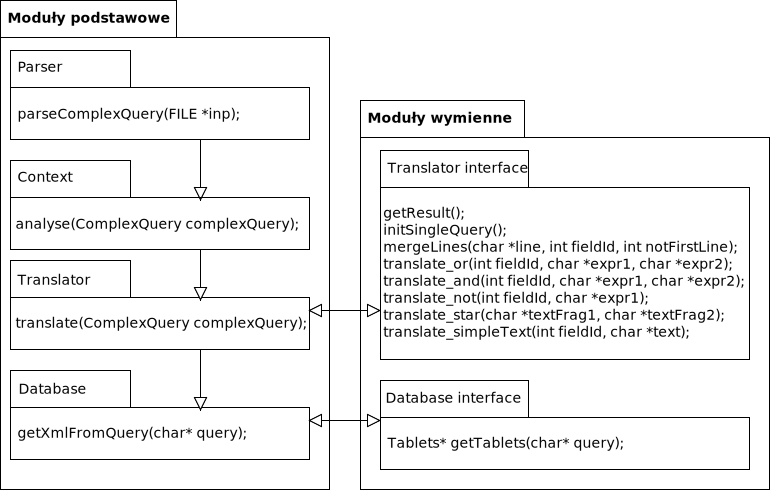
\includegraphics[width=450px]{../diagramy/pakiety.pdf}
 % pakiety.pdf: 585x300 pixel, 72dpi, 20.64x10.58 cm, bb=0 0 585 300
 \caption{Podział programu na moduły}
 \label{moduly}
\end{figure}


Na rysunku \ref{struktura_systemu} przedstawiamy ogólnie strukturę systemu, który korzysta z translatora TQL. Taki system, oprócz modułów podstawowych translatora, zawiera bazę tabliczek w dowolnej formie, implemetację modułów wymiennych umożliwiającą korzystanie z tej bazy, oraz interfejs użytkownika - do wprowadzania zapytań i wyświetlania wyników. \\

 W niniejszej pracy prezentujemy dwie prototypowe implementacje translatora, zawierające własne zestawy modułów wymiennych: 
dla bazy PostgreSQL oraz XML.
%TODO: przeformułować (moduły wymienne na poziomie kompilacji)
   Wybór modułów wymiennych odbywa się na poziomie kompilacji. Jest to rozwiązanie najprostsze do zaimplementowania,
  jednak wymaga osobnego programu dla każdego rodzaju bazy danych.

 Stworzony przez nas Makefile domyślnie buduje obie implementacje translatora TQL.
%Bez względu na wybór modułu wymiennego interfejs całego translatora jest taki sam we wszystkich instancjach.

\begin{figure}[h]
 \centering
 \includegraphics[width=450px,bb=0 0 608 517]{../diagramy/struktura2.pdf}
 % struktura.pdf: 608x517 pixel, 72dpi, 21.45x18.24 cm, bb=0 0 608 517
 \caption{Struktura systemu korzystającego z translatora}
 \label{struktura_systemu}
\end{figure}

\chapter{Moduły podstawowe}

W tym rozdziale przedstawimy dokładniej poszczególne moduły podstawowe translatora.

\section{Parser}
Parser został utworzony za pomocą narzędzia BNFC \cite{bnfc}. Na podstawie etykietowanej gramatyki BNF 
narzędzie to tworzy parser oraz szkielet analizatora składni w wybranym języku: C, C++, C\#, F\#, Haskell, Java lub OCaml. 
BNFC tworzy również pliki wejściowe dla generatora leksera (np. Flex) oraz dla generatora parsera (np. Bison). 
Dodatkowym produktem jest dokument w formacie Latex, który zawiera specyfikację zaprojektowanego języka.


Po automatycznym utworzeniu parsera, 
poprawiłyśmy nazwy stałych oznaczających symbole na bardziej intuicyjne.
Następnie
dodałyśmy tablicę symboli,
usunęłyśmy niepotrzebne funkcje z interfejsu
i ogólnie uporządkowałyśmy kod.

Moduł  parsuje zapytanie w języku TQL, tworząc drzewo struktury składniowej, które jest zdefiniowane w pliku pomocniczym Absyn.h.

Główna funkcja tego modułu to \verb|parseComplexQuery(FILE *inp)|. Argumentem jest wskaźnik do pliku zawierającego zapytanie TQL, 
a wynikiem odpowiednie drzewo struktury składniowej.

Na parser składają się następujące pliki:
\begin{itemize}
 \item Parser.cpp
 \item Parser.h
 \item TQL.y % tłumaczony na Parser.c
 \item TQL.l % tłumaczony na Lexer.c
\end{itemize}


\section{Analizator kontekstowy}
Podstawową funkcją w tym module jest \verb|analyse(ComplexQuery complexQuery)|, której argumentem oraz wynikiem jest 
drzewo struktury składniowej zapytania TQL. Funkcja ta
 sprawdza, czy podano prawidłowe nazwy pól, na podstawie których następuje wyszkukiwanie,  %to co jest po lewej w linii zapytania jest nazwą pola.
oraz upraszcza drzewo - z wywołania zapytania (wywołanie \textit{search in}) tworzy zapytanie proste.

Analizator kontekstowy składa się z następujących plików:
\begin{itemize}
 \item Context.cpp
 \item Context.h
\end{itemize}

\section{Translator}
Zadaniem translatora jest przetłumaczenie drzewa składni abstrakcyjnej na zapytanie w docelowym języku.
Składa się z następujących plików:
\begin {itemize}
 \item Translator.cpp
 \item Translator.h
 \item Translator\_interface.h (interfejs modułu translatora zależnego od bazy danych)
 %\item Translator\_config.c (implementacja interfejsu z Translator\_config.h, zależny od wyboru bazy danych itp)
\end {itemize}

Tłumaczenie poszczególnych elementów drzewa zależy od implementacji interfejsu zawartego w pliku Translator\_interface.h. 
Funkcja \verb|translate(ComplexQuery complexQuery)| przechodzi całą strukturę drzewa, wywołując w razie 
potrzeby odpowiednie funkcje z Translator\_interface.
Następnie pobiera przetłumaczone zapytanie za pomocą funkcji getResult() i przekazuje je jako wynik.

\section{Baza}
Moduł bazy jest odpowiedzialny za wywołanie przetłumaczonego zapytania i przekazanie wyniku w określonej formie - jako XML.
Składa się z następujących plików:
\begin {itemize}
 \item Database.cpp
 \item Database.h
 \item Database\_interface.h (interfejs modułu bazy zależnego od bazy danych)
% \item Database\_config.c (implementacja interfejsu z Database\_conf.h, zależny od wyboru bazy danych itp)
\end {itemize}

Główną funkcją w tym module jest \verb|getXmlFromQuery(char *query)|, która
wywołuje funkcję \verb|getTablets(char *query|) z Database\_interface.h, jako parametr podając przetłumaczoną treść zapytania. 
Dostaje w wyniku strukturę danych Tablets, wypełnioną informacjami o wyszukanych tabliczkach.
Następnie na podstawie otrzymanej struktury tworzy dokument XML i przekazuje go jako wynik wywołania zapytania.
\newline
Struktura Tablets zawiera metadane tabliczki, jej treść oraz informację o frazach, na podstawie których tabliczka została znaleziona. 
Poniżej przedstawiamy definicję struktury Tablets:
\begin{verbatim}
typedef struct{    
    char* id;
    char* id_cdli;
    char* publication;
    char* measurements;
    char* year;
    char* provenience;
    char* period;
    char* genre;
    char* subgenre;
    char* collection;
    char* text;
    Tags* tags; // specjalnie oznaczone miejsca w tekscie - frazy wyszukiwania
} Tablet;

typedef struct{
    int size;
    Tablet* tabs;
} Tablets;
\end{verbatim}

% TODO: czy tak jest ok?
Zakładamy, że w bazie danych znajdują się informacje potrzebne do wypełnienia powyższej struktury.
%Wszystkie niezbędne informacje powinny się znajdować w bazie danych.

\section{Pliki pomocnicze}
Definicje struktur danych i funkcji służących do budowy drzewa struktury składniowej (wygenerowane za pomocą BNFC \cite{bnfc}, 
następnie uproszczone):
\begin{itemize}
 \item Absyn.cpp
 \item Absyn.h
\end{itemize}
Tablica symboli:
\begin{itemize}
 \item Symbols.cpp
\item Symbols.h
\end{itemize}
Obsługa błędów:
\begin{itemize}
 \item Err.cpp
\item Err.h
\end{itemize}
Moduł do dzielenia tekstu względem separatora, pobrany z internetu \cite{cexplode}:
\begin{itemize}
 \item Cexplode.cpp
 \item Cexplode.h
\end{itemize}


\chapter{Moduły wymienne}
Pliki zależne od wyboru konkretnej bazy danych to:
\begin{itemize}
 \item Translator\_$<$nazwa$>$.cpp - dla modułu translatora
\item Database\_$<$nazwa$>$.cpp - dla modułu bazy
\end{itemize}
Ich interfejsy są wspólne dla wszystkich baz danych.

\section{Baza PostgreSQL}
\subsection{Diagram encji}
\begin{figure}[h]
 \centering
 \includegraphics[width=500px,bb=0 0 930 560]{../diagramy/diagram-encji-maly.pdf}
 % diagram-encji-maly.pdf: 930x560 pixel, 72dpi, 32.81x19.76 cm, bb=0 0 930 560
 \caption{Diagram encji}
\end{figure}
Jednym z problemów przy projektowaniu bazy danych był wybór takiej reprezentacji treści tabliczki, 
żeby efektywnie wyszukiwać zarówno treść konkretnej tabliczki jak i tabliczki, których treść spełnia podane kryteria
 (wg odczytów lub zapisu klinowego).

W przypadku pierwszego problemu jako rozwiązanie narzuca się przechowywanie treści
jako otwarty tekst.
Natomiast najlepszym rozwiązaniem drugiego jest reprezentacja treści tabliczki
w formie grafu, którego krawędziami są odczyty i kliny (zgodnie z pomysłem dr Wojciecha Jaworskiego\cite[s.13-24]{jaworski}).
Zdecydowałyśmy się na połączenie obu sposobów. Odczyty oraz kliny przechowujemy w tabelach Reading i Cuneiform, 
natomiast otwarty tekst w kolumnie show\_text tabeli Tablet. 
% TODO: dwie reprezentacje - jeszcze przejrzeć
% nie wiadomo po co jest odwzorowanie
Dzięki temu rozwiązaniu, szukając tabliczki zawierającej podane odczyty (lub kliny) korzystamy z reprezentacji
grafowej w tabelce Reading (lub Cuneiform).
Natomiast zawsze korzystamy z reprezentacji otwartym tekstem w tabelce Tablet w celu wyświetlenia treści tabliczki.
Aby zapewnić możliwość odwzorowania treści tabliczki między reprezentacjami, węzły są liczbami postaci:
\begin{verbatim}
 <numer węzła w tabliczce> * 1 000 000 + <id tabliczki>
\end{verbatim}
gdzie numer węzła w tabliczce to numer kolejnego słowa (słowa są oddzielone spacjami i końcem linii) pomnożone przez 10 
(żeby umożliwić wstawienie kilku węzłów w jednym słowie np. pozwolić na przetłumaczenie jednego słowa na sekwencję trzech klinów). 


Przerywane linie na diagramie encji oznaczają opisany powyżej związek pomiędzy id węzła (node1\_id i node2\_id) 
a id tabliczki (Tablet.id).

% relacja
% Stąd wzięły się przerywane linie na diagramie encji - nie ma bezpośredniego klucza obcego w tabeli Reading (czy Tag) do Tablet, 
% jednak związek istnieje. Taki sposób przechowywania informacji o treści tabliczki umożliwia sprawniejsze wyszukiwanie nie tylko
% po odczytach (pozwala pomijać linie z uszkodzeniami) ale także w przyszłości ułatwia zaimplementowanie wyszukiwania po klinach,
% po tagach itp.
% Poza sprawnym
%  wyszukiwaniem ułatwia to rozszerzenie programu o możliwość wyszukiwania po klinach - po dodaniu tabeli Cuneiform.

 

\subsection{Translator\_postgres}
Tłumaczy otrzymane fragmenty drzewa struktury zapytania na język SQL. Przetłumaczone fragmenty zbiera do buforów 
(\textit{select}, \textit{from}, \textit{where}), które następnie odpowiednio łączy.
Każde proste zapytanie TQL jest tłumaczone na pojedyncze zapytanie SQL. Tłumaczenie kilku prostych zapytań
łączone jest za pomocą UNION.

\subsubsection{Stałe fragmenty zapytania}
Tłumaczenie prostego zapytania zaczyna się od inicjalizacji buforów przechowujących poszczególne części wynikowego SQL-a.\\
\textit{select} jest inicjowany na 
\begin{verbatim}
SELECT t.id, t.id_cdli, t.publication, t.measurements, t.origin_date, 
       p.value as provenience, pd.value as period,
       g1.value as genre, g2.value as subgenre, 
       c.value as collection, t.text
\end{verbatim}
\textit{from} jest inicjowany
\begin{verbatim}
FROM tablet t
  LEFT JOIN provenience p ON p.id = t.provenience_id
  LEFT JOIN collection c ON c.id = t.collection_id
  LEFT JOIN genre g1 ON g1.id = t.genre_id
  LEFT JOIN genre g2 ON g2.id = t.subgenre_id
  LEFT JOIN period pd ON pd.id = t.period_id
\end{verbatim}
\textit{where} początkowo zawiera pusty ciąg znaków.



\subsubsection{Tłumaczenie zapytań o atrybuty tabliczki}
Poniższe tłumaczenia są dodawane do bufora \textit{where} i łączone za pomocą AND.
\begin{longtable}{|p{3in}|p{3in}|}
\hline
{\bf Konstrukcja} & {\bf Tłumaczenie na SQL}\\
\hline
\endhead
provenience: wartosc & \begin{verbatim}p.value LIKE 'wartosc'\end{verbatim}
\\
\hline
publication: wartosc & 
\begin{verbatim}
t.publication LIKE 'wartosc'
\end{verbatim}
\\
\hline
period: wartosc & 
\begin{verbatim}
pd.value LIKE 'wartosc'
\end{verbatim}
\\
\hline
year: wartosc & 
\begin{verbatim}
t.origin_date LIKE 'wartosc'
\end{verbatim}
\\
\hline
genre: wartosc & 
\begin{verbatim}
   g1.value LIKE 'wartosc' 
OR g2.value LIKE 'wartosc'
\end{verbatim}
\\
\hline
cdli\_id: wartosc & 
\begin{verbatim}
t.cdli_id LIKE 'wartosc'
\end{verbatim}
\\
\hline
museum: wartosc & 
\begin{verbatim}
t.museum LIKE 'wartosc'
\end{verbatim}
\\
\hline
collection: wartosc & 
\begin{verbatim}
c.value LIKE 'wartosc'
\end{verbatim}
\\
\hline
\end{longtable}

\textbf{Tłumaczenie operatorów:}
\begin{longtable}{|p{1in}|p{1in}|}
\hline
{\bf Operator} & {\bf Tłumaczenie}\\
\hline
\endhead
/ & OR\\ 
\hline
-- & NOT\\ 
\hline
+ & AND\\ 
\hline
* & \%  \\ 
\hline
\end{longtable}


\subsubsection{Tłumaczenie zapytań o treść tabliczki}
Przy tłumaczeniu zapytań o treść tabliczki
korzystamy z przedstawienia treści tabliczki w formie grafu.

Pojawienie się wyszukiwania po treści tabliczki niesie za sobą konieczność dodania do bufora \textit{from}:
\begin{verbatim}
INNER JOIN (
  <wynikowe zapytanie o treść tablczki>
) AS sequence ON sequence.id_tab = t.id
\end{verbatim}

natomiast do \textit{select} dodajemy:
\begin{verbatim}
, sequence.nodes as nodes
\end{verbatim}

gdzie $<$wynikowe zapytanie o treść tablczki$>$ to kombinacja zapytań typu:
\begin{verbatim}
  SELECT 
    id_tab, 
    CAST(array_accum(nodes) as TEXT) as nodes, 
    COUNT(DISTINCT id_seq) AS seq, 
    <id_sekw> AS id_seq
  FROM (
    SELECT
      t1.node1_id % 1000000 AS id_tab,
      '{' || t1.node1_id || ',' || t<dl_sekw>.node2_id || '}' AS nodes,
      1 AS id_seq
    FROM
      <nazwa_tabeli> t1
      LEFT JOIN <nazwa_tabeli> t2 ON (t2.node1 = t1.node2)
      LEFT JOIN <nazwa_tabeli> t3 ON (t3.node1 = t2.node2)
      ...
      LEFT JOIN <nazwa_tabeli> t<dl_sekw> ON (t<dl_sekw>.node1 = t<dl_sekw-1>.node2)
   WHERE
      t1.value LIKE '<sekw[1]>'
     AND
      t2.value LIKE '<sekw[2]>'
    AND
      t3.value LIKE '<sekw[3]>'
    AND
      ...
    AND
      t<dl_sekw>.value LIKE '<sekw[<dl_sekw>]>'
   ) AS a 
  GROUP BY id_tab
\end{verbatim}
Zmienne użyte w powyższym pseudo-kodzie:
\begin{description}
 \item[id\_sekw] - kolejny numer sekwencji (przydatny przy bardziej skomplikowanym zapytaniu - do rozróżniania podzapytań)
 \item[dl\_sekw] - ilość słów składających się na wyszukiwaną sekwencję
 \item[sekw] - tablica zawierająca słowa składające się na wyszukiwaną sekwencję
\item[nazwa\_tabeli] - nazwa tabeli, w której wyszukujemy (Reading lub Cuneiform)
 \end{description}

\begin{longtable}{|p{1in}|p{4.5in}|}
\hline
{\bf Operator} & {\bf Tłumaczenie}\\
\hline
\endhead
/ & 
\begin{verbatim}
SELECT 
  id_tab, 
  CAST(array_accum(nodes) as TEXT) as nodes, 
  COUNT(DISTINCT id_seq) as seq,
  <id_sekw> as id_seq
FROM 
(
  <zapytanie1>
  UNION
  <zapytanie2>
)
as c
GROUP BY id_tab
\end{verbatim}
\\ 
\hline
+ &
\begin{verbatim}
SELECT * FROM
 (SELECT id_tab, 
         CAST(array_accum(nodes) as TEXT) as nodes, 
         COUNT(DISTINCT id_seq) as seq, 
         <id_sekw> as id_seq
  FROM
    (<zapytanie1>
    UNION
    <zapytanie2>)
  as c 
  GROUP BY id_tab
 ) as b
WHERE b.seq=2 
\end{verbatim}
\\ 
\hline
-- & 
\begin{verbatim}
SELECT 
  id_tab, 
  '' as nodes, 
  0 as seq,
  <id_sekw> as id_seq
FROM
(
 (SELECT id as id_tab from tablet)
 EXCEPT
 (SELECT id_tab from
    <zapytanie_negowane> as a
 )   
) as b
\end{verbatim}
\\ 
\hline
* & \%  \\ 
\hline
\end{longtable}


\subsection{Database\_postgres}

Odpowiada za wywołanie zapytania w konkretnej bazie i zapisanie wyniku do struktury Tablets.
 Korzysta z pliku database.conf, który zawiera dane dostępu do bazy (nazwa bazy, host, port, użytkownik, hasło)
oraz biblioteki libpq-fe.h do PostgreSQL.

\subsection{Baza XML}
W budowie :)
%\chapter{Dokumentacja użytkowa i opis implementacji}\label{r:impl}
%\chapter{Dokumentacja użytkowa i opis implementacji}\label{r:impl}
\chapter*{Podsumowanie}
\addcontentsline{toc}{chapter}{Podsumowanie}
% Zakończenie pracy magisterskiej jest jej podsumowaniem, w którym powinno się znaleźć potwierdzenie 
% lub też obalenie założonej przez autora tezy, poparte odpowiednimi argumentami. 
% Zamieścić tu można również pewien bilans swojej pracy oraz wszelkie nasuwające się wnioski. 
% Zakończenie ma postać klamry, spinającej całą pracę magisterską w pewną całość składającą się ze wstępu, 
% rozwinięcia oraz zakończenia, które stanowi konkluzję dla całej pracy.
% 
% W zakończeniu powinno się zamieścić kilka zdań od siebie, na przykład dotyczących prognozy analizowanego zjawiska, 
% rokować, wątpliwości itp. Tak jak i we wstępie, również tutaj autor powinien popisać się niejako swoimi umiejętnościami 
% pisarskimi, erudycją i kompetencjami w opisywanej dziedzinie, istnieje bowiem duże ryzyko, iż właśnie zakończenie zostanie 
% przeczytane przez recenzenta.

\section*{Podsumowanie projektu}
\addcontentsline{toc}{section}{Podsumowanie projektu}
%cel osiągnięty
Przedstawiona w niniejszej pracy realizacja języka TQL spełnia najważniejsze postulaty. 
Po pierwsze jest on intuicyjny i prosty w użyciu dla osób znających jedynie dziedzinę problemu.
% (co potwierdza opinia dr hab. Marka Stępnia)
Po drugie minimalnie ogranicza siłę wyrazu pozwalając na tworzenie skomplikowanych zapytań.

%wady
Język TQL ma jednak kilka ograniczeń w stosunku do typowych języków zapytań. 
Największym z nich jest brak wpływu na postać wyniku, co utrudnia np. zbieranie danych statystycznych 
(m. in. nie da się spytać o ilość tabliczek spełniających dane kryteria). 
Można jednak stworzyć narzędzia do samej prezentacji wyników zapytań, które pokonają to ograniczenie. 

Należy pamiętać, że TQL jest jedynie językiem wyszukiwania -- w przeciwieństwie do wielu innych języków zapytań
nie udostępnia możliwości zmieniania danych znajdujących się w bazie, ani dodawania nowych. 

%zalety
Dzięki specyficznym cechom języka TQL, można również dostosować go do wykorzystania w innych dziedzinach. 
Należy tu wspomnieć o braku ograniczenia ilości i nazw pól, po których można wyszukiwać oraz przystosowaniu 
do wyszukiwania wg kryteriów dotyczących danych tekstowych. 
Na podstawie TQL można łatwo stworzyć rodzinę języków dla różnych dziedzin zajmujących się przeszukiwaniem tekstów.

%luźne uwagi
W ramach niniejszej pracy zaprezentowane zostały dwie implementacje języka TQL. 
Po stworzeniu pierwszej czas poświęcony na drugą był już niewielki. 
Największym zadaniem było przetłumaczenie poszczególnych konstrukcji TQL na XQuery. 
Pozwala to sądzić, że każda kolejna implementacja, dla różnych typów baz i różnych schematów danych, 
nie będzie wymagała dużego nakładu pracy. 

\pagebreak

\section*{Możliwości rozwoju}
\addcontentsline{toc}{section}{Możliwości rozwoju}
\begin{figure}[h]
 \centering
 \includegraphics[width=500px]{../diagramy/wyszuk_zapyt.png}
 % wyszuk_zapyt.png: 811x524 pixel, 72dpi, 28.61x18.49 cm, bb=0 0 811 524
 \caption{Okno do wprowadzania zapytania}
 \label{fig:wyszuk_zapyt}
\end{figure}

\begin{figure}[h]
 \centering
 \includegraphics[width=500px]{../diagramy/wyszuk_wynik.png}
 % wyszuk_wynik.png: 823x628 pixel, 72dpi, 29.03x22.15 cm, bb=0 0 823 628
 \caption{Sposób prezentacji wyników zapytania}
 \label{fig:wyszuk_wynik}
\end{figure}

%co dalej
Jako dodatek do pracy stworzyłyśmy stronę internetową umożliwiającą zadanie zapytania w języku TQL i prezentującą wyniki. 
Jej wygląd jest przedstawiony na rysunkach \ref{fig:wyszuk_zapyt} oraz \ref{fig:wyszuk_wynik}.
% TODO: W chwili obecnej jest ona dostępna na stronie \url{http://students.mimuw.edu.pl/~/jw234694/sumlib/}.
Stanowi ona zalążek przyjaznego interfejsu użytkownika dla naukowców, którzy będą współpracować z TQL. Plany jej rozwoju
uwzględniają między innymi funkcjonalność graficznego budowanie zapytania.
% TODO: walnąć rozdzialik o graficznym bilderze
Na chwilę obecną serwis internetowy jest w trakcie udostępniania Wydziałowi Historii UW.
Pracownicy tej instytucji będą pierwszymi testerami całego rozwiązania.

Poza tym warto nawiązać współpracę z projektem CDLI, (zob. rozdział \ref{chapter:cdli}).
Implementacja TQL dla bazy CDLI, wraz z interfejsem www, z pewnością byłaby przydatnym narzędziem dla sumerologów na całym świecie.

W dalszej perspektywie można rozwinąć język TQL między innymi o wyszukiwanie wg klinów i wg tagów. 
Pierwsze z nich wymaga przetłumaczenia odczytów na kliny oraz umieszczenia tych informacji w bazie danych.
Drugie natomiast potrzebuje narzędzia do wykrywania poszczególnych tagów
(postaci, miar, dat, liczb itp) lub do ich zaznaczania przez sumerologów.

Dodatkowo warto stworzyć narzędzie do analizy uszkodzonych fragmentów i wykrywania błędów w odczytach tekstów. 
Dzięki niemu można by zmniejszyć ryzyko pominięcia istotnych tabliczek podczas wyszukiwania. 

Rozwój projektu będzie zależał również od potrzeb zgłaszanych przez samych sumerologów.







\appendix

\chapter{Schemat bazy danych xml}


\include{pliki/sumlib_xs}





\begin{thebibliography}{99}
\addcontentsline{toc}{chapter}{Bibliografia}
\bibitem[1]{jaworski} Wojciech Jaworski, \textit{Modelowanie tresci sumeryjskich tekstów gospodarczych z epoki Ur~III}, 
\url{http://nlp.ipipan.waw.pl/NLP-SEMINAR/071119.pdf}, 19 listopada 2007
\bibitem[2]{cexplode} \url{http://maz-programmersdiary.blogspot.com/2008/09/c-explode.html}



%\bibitem[Bea65]{beaman} Juliusz Beaman, \textit{Morbidity of the Jolly
 %   function}, Mathematica Absurdica, 117 (1965) 338--9.

\end{thebibliography}

\listoffigures

\end{document}


%%% Local Variables:
%%% mode: latex
%%% TeX-master: t
%%% coding: latin-2
%%% End:
